\documentclass[germanthesis,twoside,modernchapter]{i4thesis}
% options:
% [germanthesis] - Thesis is written in German
% [plainunnumbered] - Don't print numbers on plain pages
% [earlydraft] - Settings for quick draft printouts
% [watermark] - Print current time/date at bottom of each page
% [phdthesis] - switch to PhD thesis style
% [modernchapter] - modern chapter headings
% [twoside] - double sided

\usepackage{dataref}
\drefset{/experiment 1/a}{21}
\drefset{/experiment 1/base}{105}



\bibliography{references}

\author{Toller Student}
\title{Über das Verhältnis zwischen Bachelorarbeit und resultierender Note}
\thesistype{Bachelorarbeit im Fach Informatik}
\thesiscite{Bachelor's Thesis}
\birthday{1. Dezember 1985}
\birthplace{Hier}
\thesisstart{1. Februar 2014}
\thesisend{1. August 2014}
\advisors{& \textbf{Dipl.-Inf.~Marianne Mustermann}\\
& \textbf{Max Mustermann, M.Sc.}\\}

\begin{document}

\pagenumbering{roman}

\maketitle

\chapter*{Abstract}
\addcontentsline{toc}{chapter}{Abstract}
\begin{otherlanguage*}{american}

about 1/2 page:   \\
(1) Motivation (Why do we care?)   \\
(2) Problem statement (What problem are we trying to solve?)   \\
(3) Approach (How did we go about it)   \\
(4) Results (What's the answer?)   \\
(5) Conclusion (What are the implications of the answer?)

\end{otherlanguage*}


\chapter*{Kurzfassung}
\addcontentsline{toc}{chapter}{Kurzfassung}
\begin{otherlanguage*}{ngerman}

Gleicher Text in Deutsch

\end{otherlanguage*}

\acresetall

\cleardoublepage
\tableofcontents

\cleardoublepage
\pagenumbering{arabic}

\chapter{Introduction}
%\chapter{Einleitung}
\label{sec:introduction}

general motivation for your work, context and goals: 1-2 pages

\begin{itemize}
\item \textbf{Context:} make sure to link where your work fits in
\item \textbf{Problem:} gap in knowledge, too expensive, too slow, a deficiency, superseded technology
\item \textbf{Strategy:} the way you will address the problem 
\end{itemize}


\section{Sample Section}

The following samples explain how to insert cross-references, figures and tables, how to set math, algorithms and program code, how to add references, and how to use acronyms.


\subsection{Cross References}
\label{sec:cross-ref}

Use the \verb|\label| and \verb|\cref| commands for cross references, e.g.\ to \cref{sec:cross-ref}. 

\subsection{Figures}

\Cref{fig:setup0} shows the distribution of the nodes in the sample setup at time $t=0$, as well as the initial coverage with a sensing radius of \SI{30}{\metre} and the communication graph for a communication range of \SI{50}{\metre}.
Figure captions should always be placed at the bottom of the figure.

\begin{figure}
	\centering
	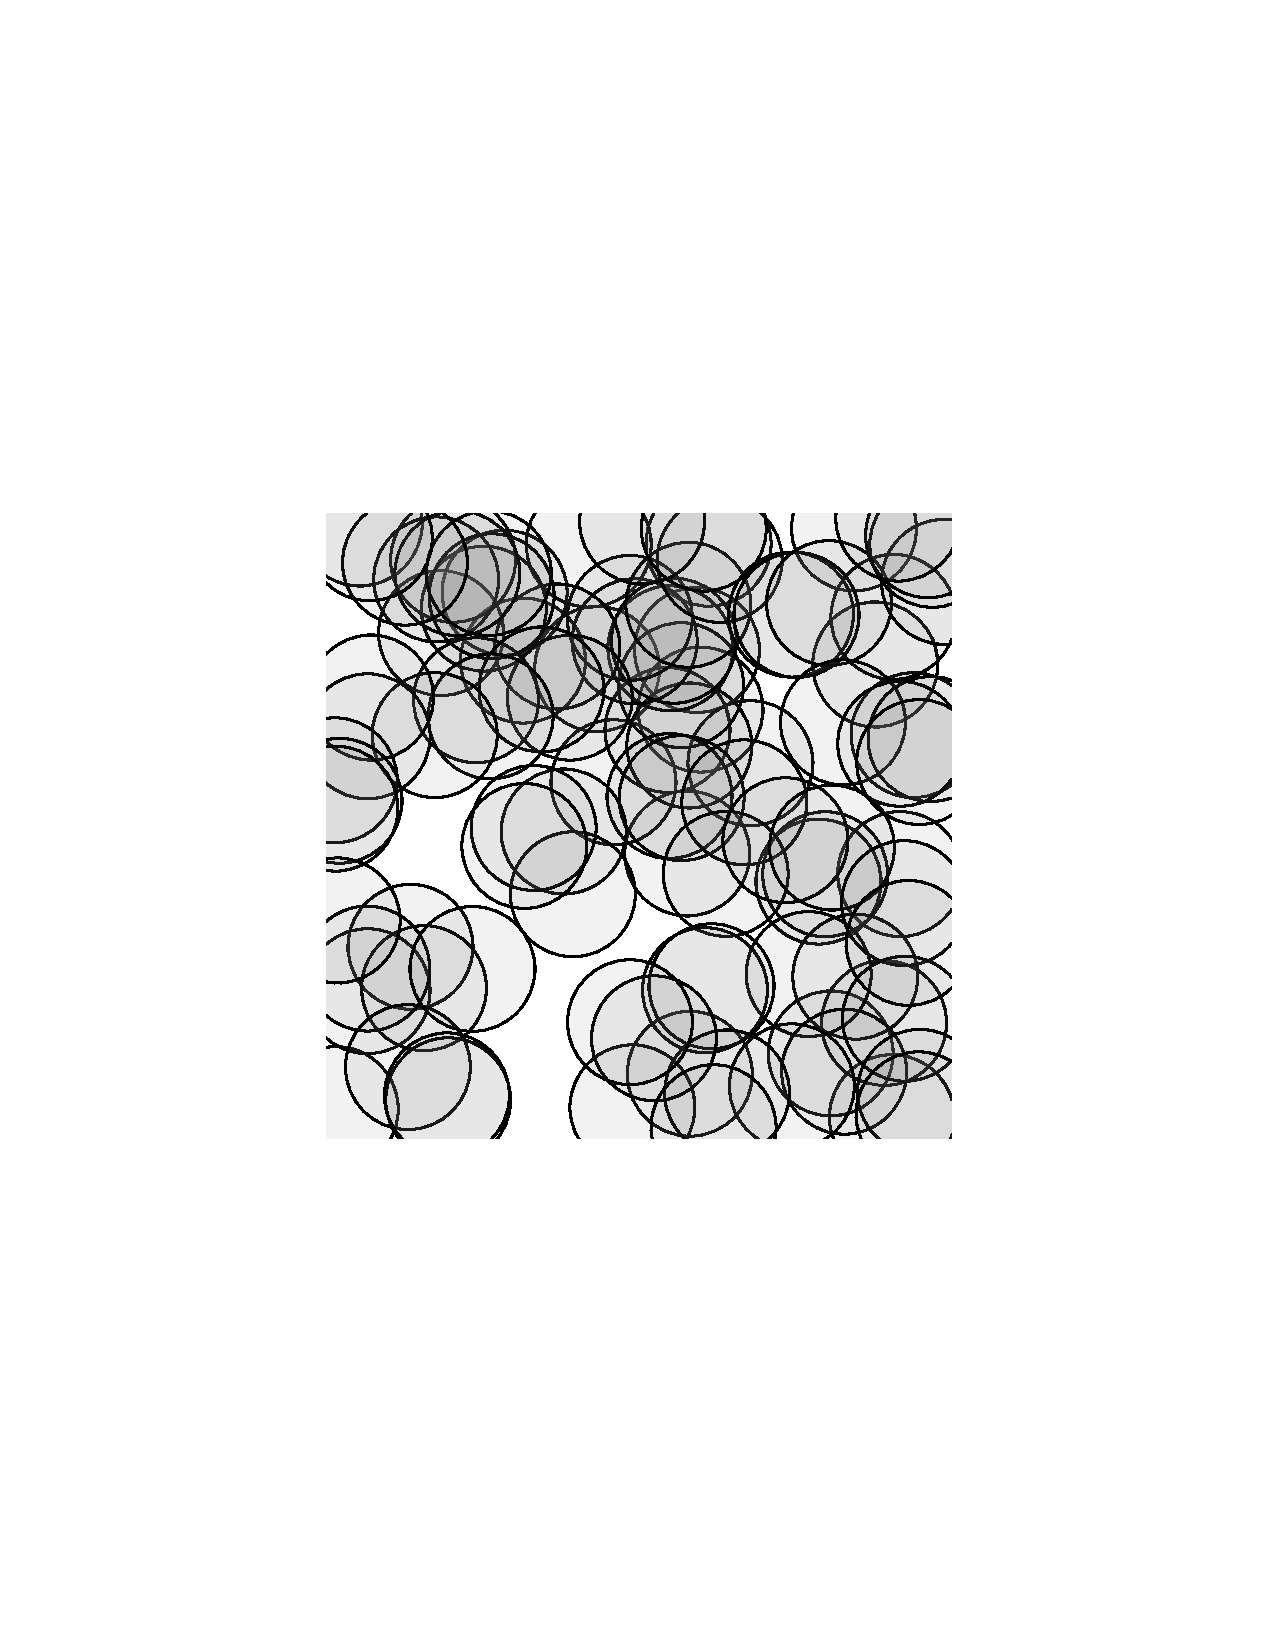
\includegraphics[width=0.3\textwidth]{figures/coverage-30--0-static1}
	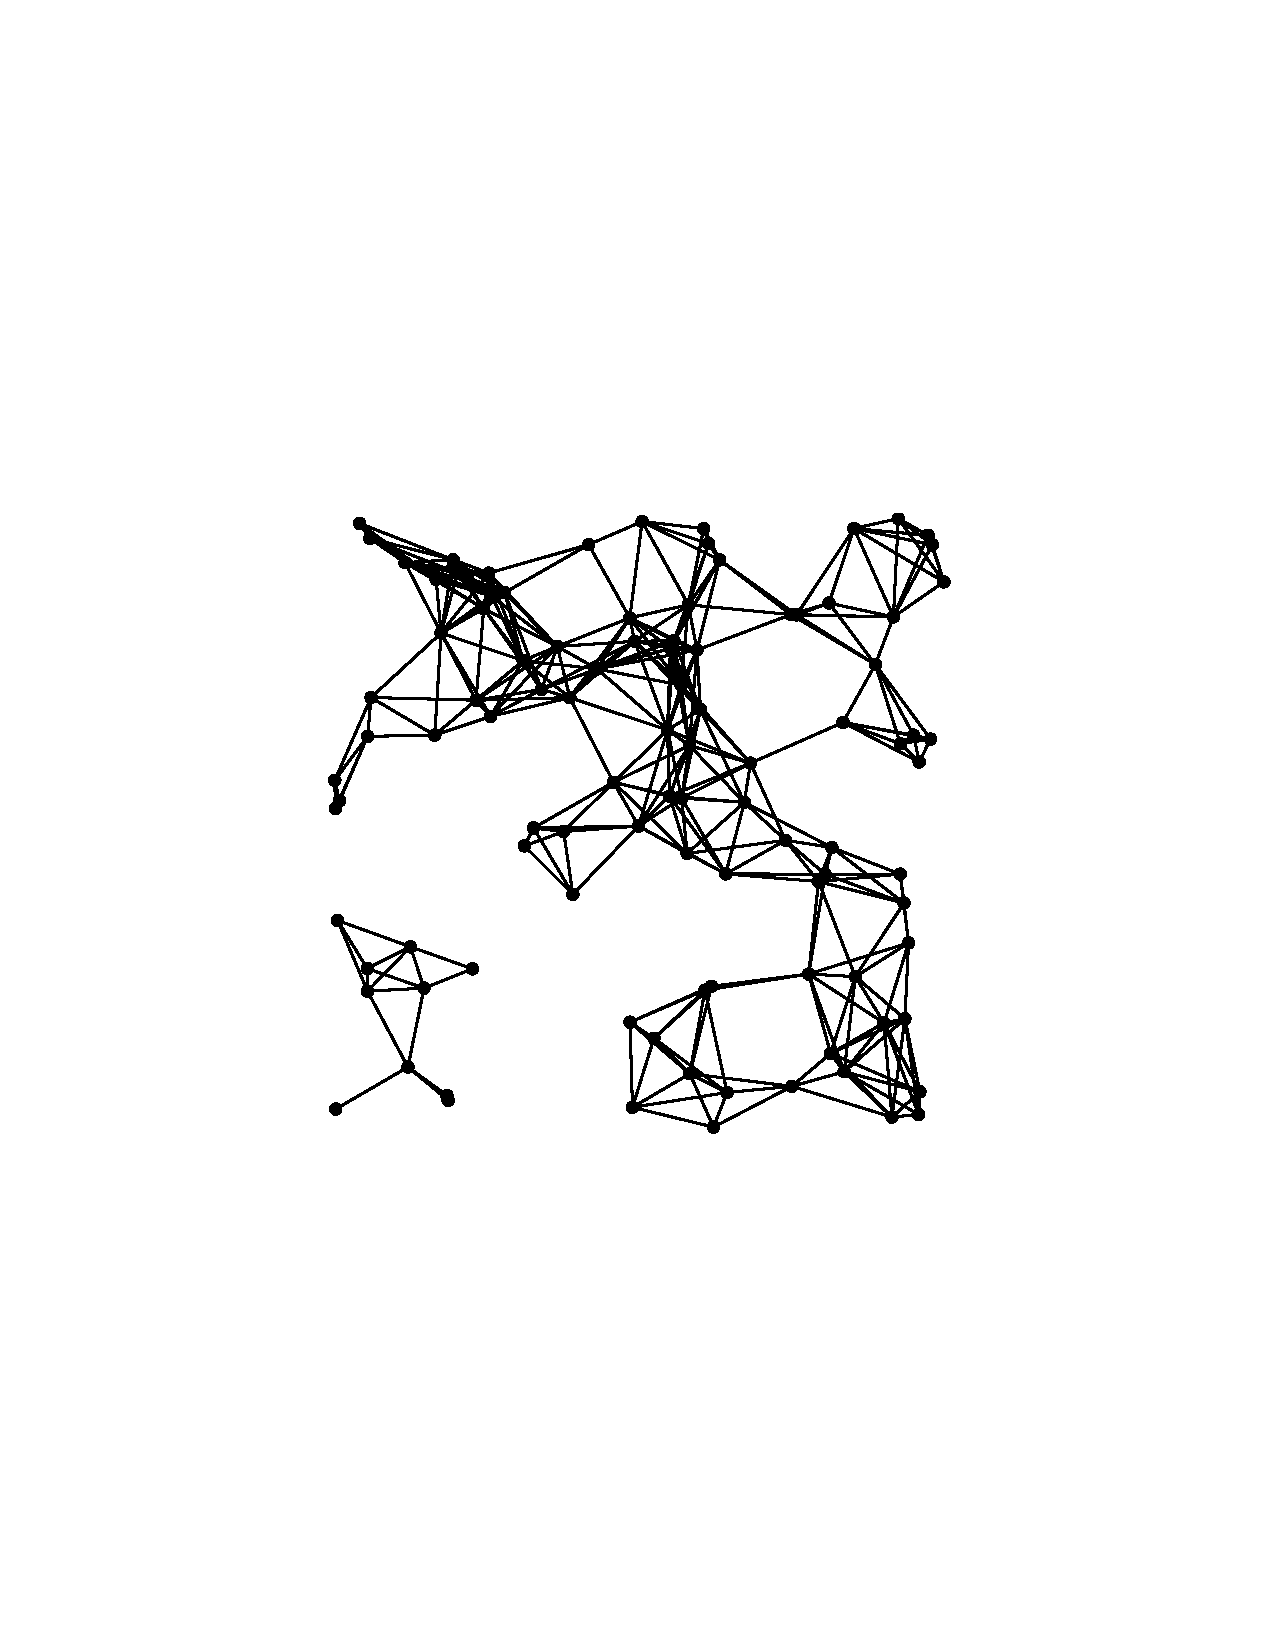
\includegraphics[width=0.3\textwidth]{figures/connectivity-50-0-static1}
	\caption{Coverage and connectivity for a sample replication at time $t=0$}
	\label{fig:setup0}
\end{figure}

\subsection{Subfigures}

\Crefrange{fig:setup1}{fig:setup2} show the distribution of the nodes in the sample setup at time $t=0$, as well as the initial coverage with a sensing radius of \SI{30}{\metre} and the communication graph for a communication range of \SI{50}{\metre}.

\begin{figure}%
	\centering
    \begin{subfigure}{0.3\textwidth}
      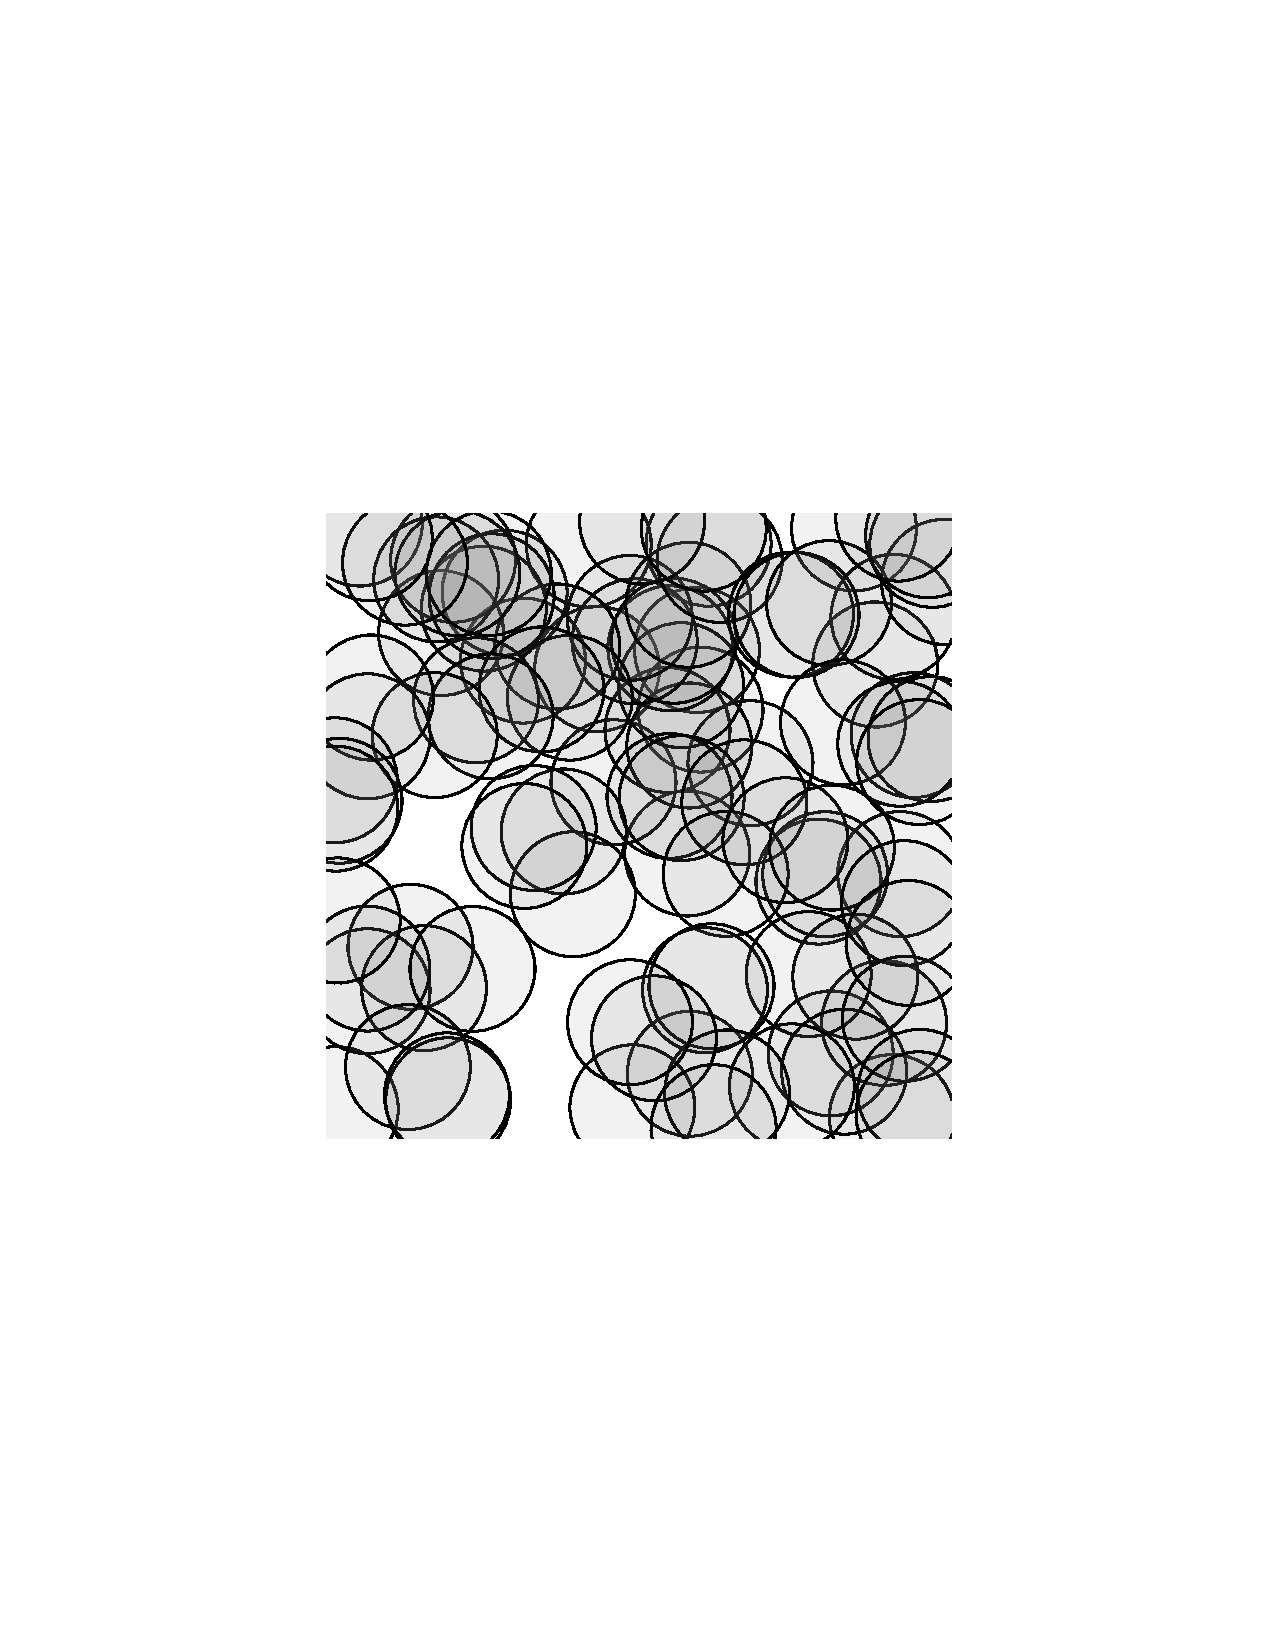
\includegraphics[width=\textwidth]{figures/coverage-30--0-static1}
      \caption{coverage}\label{fig:setup1}
    \end{subfigure}
    \begin{subfigure}{0.3\textwidth}
      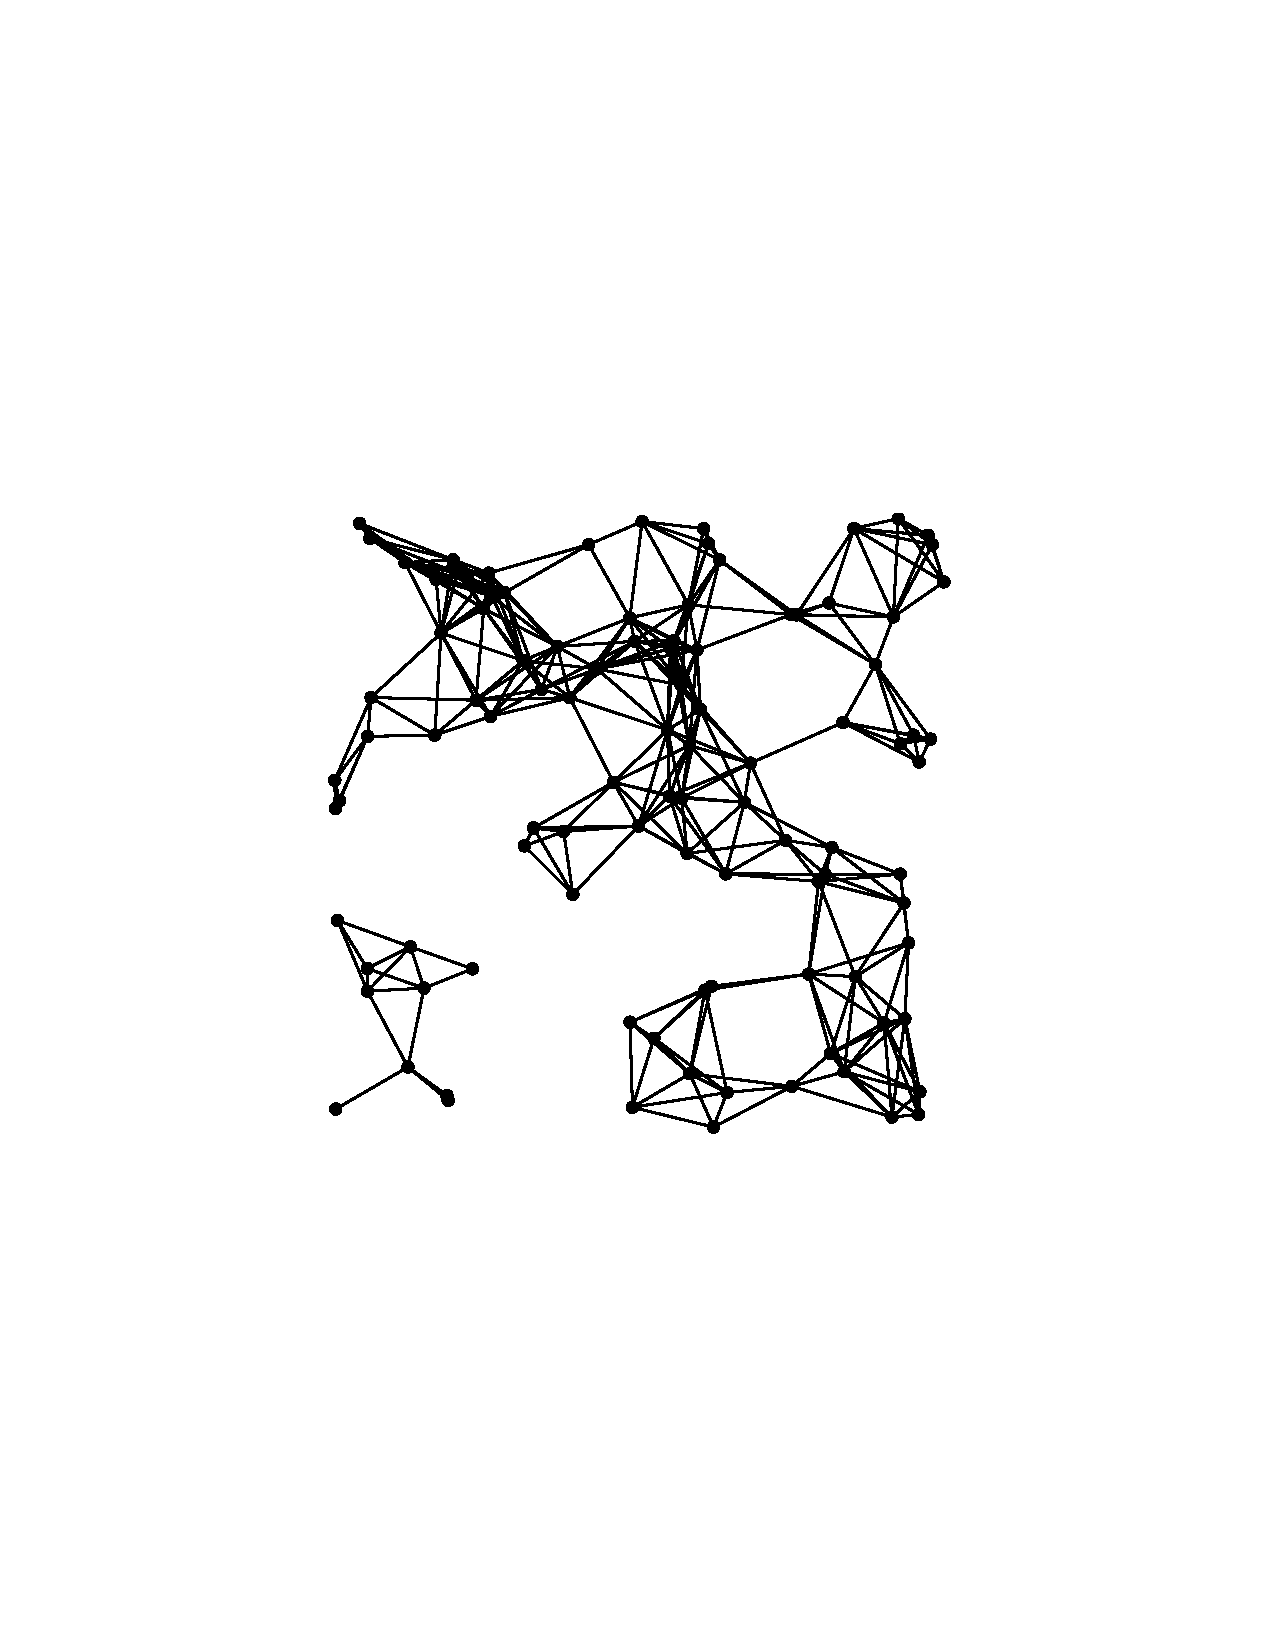
\includegraphics[width=\textwidth]{figures/connectivity-50-0-static1}
      \caption{connectivity}\label{fig:setup2}
    \end{subfigure}
	\caption{Subfigures showing coverage and connectivity for a sample replication at time $t=0$}%
	\label{fig:setups12}%
\end{figure}

\ifthenelse{\boolean{gnuplot}}{
\subsection{Plotting}
You can make \LaTeX{} generate plots automatically using \texttt{gnuplot}.
Just put your data into a \texttt{csv} file in the \texttt{plots} subdirectory and create a \texttt{gnuplot} script ending in \texttt{.gplt}.
Follow the example from \texttt{plots/ass\_granularity.gplt} shown in Figure \ref{fig:AssGran}.
\begin{figure}
  \centering
  \vspace{\gnuplotpreskip}
  \tikzset{external/export=true}
  \tikzsetnextfilename{eval-ass_granularity}
  \begin{tikzpicture}[gnuplot]
%% generated with GNUPLOT 5.0p3 (Gentoo revision r0) (Lua 5.1; terminal rev. 99, script rev. 100)
%% Do 24 Mär 2016 17:09:07 CET
\tikzset{every node/.append style={font={\footnotesize}}}
\path (-1.813,-1.110) rectangle (7.187,4.890);
\gpcolor{color=gp lt color axes}
\gpsetlinetype{gp lt axes}
\gpsetdashtype{gp dt axes}
\gpsetlinewidth{0.50}
\draw[gp path] (0.000,0.000)--(6.634,0.000);
\gpcolor{color=gp lt color border}
\gpsetlinetype{gp lt border}
\gpsetdashtype{gp dt solid}
\gpsetlinewidth{1.00}
\draw[gp path] (0.000,0.000)--(-0.125,0.000);
\node[gp node right] at (-0.309,0.000) {0.0};
\gpcolor{color=gp lt color axes}
\gpsetlinetype{gp lt axes}
\gpsetdashtype{gp dt axes}
\gpsetlinewidth{0.50}
\draw[gp path] (0.000,0.822)--(6.634,0.822);
\gpcolor{color=gp lt color border}
\gpsetlinetype{gp lt border}
\gpsetdashtype{gp dt solid}
\gpsetlinewidth{1.00}
\draw[gp path] (0.000,0.822)--(-0.125,0.822);
\node[gp node right] at (-0.309,0.822) {20.0};
\gpcolor{color=gp lt color axes}
\gpsetlinetype{gp lt axes}
\gpsetdashtype{gp dt axes}
\gpsetlinewidth{0.50}
\draw[gp path] (0.000,1.644)--(6.634,1.644);
\gpcolor{color=gp lt color border}
\gpsetlinetype{gp lt border}
\gpsetdashtype{gp dt solid}
\gpsetlinewidth{1.00}
\draw[gp path] (0.000,1.644)--(-0.125,1.644);
\node[gp node right] at (-0.309,1.644) {40.0};
\gpcolor{color=gp lt color axes}
\gpsetlinetype{gp lt axes}
\gpsetdashtype{gp dt axes}
\gpsetlinewidth{0.50}
\draw[gp path] (0.000,2.466)--(6.634,2.466);
\gpcolor{color=gp lt color border}
\gpsetlinetype{gp lt border}
\gpsetdashtype{gp dt solid}
\gpsetlinewidth{1.00}
\draw[gp path] (0.000,2.466)--(-0.125,2.466);
\node[gp node right] at (-0.309,2.466) {60.0};
\gpcolor{color=gp lt color axes}
\gpsetlinetype{gp lt axes}
\gpsetdashtype{gp dt axes}
\gpsetlinewidth{0.50}
\draw[gp path] (0.000,3.288)--(6.634,3.288);
\gpcolor{color=gp lt color border}
\gpsetlinetype{gp lt border}
\gpsetdashtype{gp dt solid}
\gpsetlinewidth{1.00}
\draw[gp path] (0.000,3.288)--(-0.125,3.288);
\node[gp node right] at (-0.309,3.288) {80.0};
\gpcolor{color=gp lt color axes}
\gpsetlinetype{gp lt axes}
\gpsetdashtype{gp dt axes}
\gpsetlinewidth{0.50}
\draw[gp path] (0.000,4.110)--(3.878,4.110);
\draw[gp path] (6.450,4.110)--(6.634,4.110);
\gpcolor{color=gp lt color border}
\gpsetlinetype{gp lt border}
\gpsetdashtype{gp dt solid}
\gpsetlinewidth{1.00}
\draw[gp path] (0.000,4.110)--(-0.125,4.110);
\node[gp node right] at (-0.309,4.110) {100.0};
\draw[gp path] (0.737,0.000)--(0.737,-0.125);
\node[gp node center] at (0.737,-0.433) {2.2};
\draw[gp path] (1.474,0.000)--(1.474,-0.125);
\node[gp node center] at (1.474,-0.433) {2.4};
\draw[gp path] (2.211,0.000)--(2.211,-0.125);
\node[gp node center] at (2.211,-0.433) {2.6};
\draw[gp path] (2.948,0.000)--(2.948,-0.125);
\node[gp node center] at (2.948,-0.433) {2.8};
\draw[gp path] (3.686,0.000)--(3.686,-0.125);
\node[gp node center] at (3.686,-0.433) {3.0};
\draw[gp path] (4.423,0.000)--(4.423,-0.125);
\node[gp node center] at (4.423,-0.433) {3.2};
\draw[gp path] (5.160,0.000)--(5.160,-0.125);
\node[gp node center] at (5.160,-0.433) {3.4};
\draw[gp path] (5.897,0.000)--(5.897,-0.125);
\node[gp node center] at (5.897,-0.433) {3.6};
\draw[gp path] (0.000,4.521)--(0.000,0.000)--(6.634,0.000)--(6.634,4.521)--cycle;
\node[gp node center,rotate=-270] at (-1.567,2.260) {Schedulable Systems[\%]};
\node[gp node center] at (3.317,-0.895) {Utilisation};
\node[gp node right] at (5.166,4.187) {ABB};
\gpfill{rgb color={0.933,0.576,0.310}} (5.350,4.110)--(6.266,4.110)--(6.266,4.264)--(5.350,4.264)--cycle;
\gpfill{rgb color={0.933,0.576,0.310}} (0.484,0.000)--(0.623,0.000)--(0.623,3.925)--(0.484,3.925)--cycle;
\gpfill{rgb color={0.933,0.576,0.310}} (1.221,0.000)--(1.360,0.000)--(1.360,3.858)--(1.221,3.858)--cycle;
\gpfill{rgb color={0.933,0.576,0.310}} (1.958,0.000)--(2.097,0.000)--(2.097,3.739)--(1.958,3.739)--cycle;
\gpfill{rgb color={0.933,0.576,0.310}} (2.695,0.000)--(2.834,0.000)--(2.834,3.570)--(2.695,3.570)--cycle;
\gpfill{rgb color={0.933,0.576,0.310}} (3.432,0.000)--(3.571,0.000)--(3.571,3.432)--(3.432,3.432)--cycle;
\gpfill{rgb color={0.933,0.576,0.310}} (4.169,0.000)--(4.308,0.000)--(4.308,3.335)--(4.169,3.335)--cycle;
\gpfill{rgb color={0.933,0.576,0.310}} (4.906,0.000)--(5.046,0.000)--(5.046,3.181)--(4.906,3.181)--cycle;
\gpfill{rgb color={0.933,0.576,0.310}} (5.644,0.000)--(5.783,0.000)--(5.783,2.878)--(5.644,2.878)--cycle;
\draw[gp path] (0.553,3.901)--(0.553,3.947);
\draw[gp path] (0.484,3.901)--(0.622,3.901);
\draw[gp path] (0.484,3.947)--(0.622,3.947);
\draw[gp path] (1.290,3.830)--(1.290,3.884);
\draw[gp path] (1.221,3.830)--(1.359,3.830);
\draw[gp path] (1.221,3.884)--(1.359,3.884);
\draw[gp path] (2.027,3.705)--(2.027,3.772);
\draw[gp path] (1.958,3.705)--(2.096,3.705);
\draw[gp path] (1.958,3.772)--(2.096,3.772);
\draw[gp path] (2.764,3.530)--(2.764,3.608);
\draw[gp path] (2.695,3.530)--(2.833,3.530);
\draw[gp path] (2.695,3.608)--(2.833,3.608);
\draw[gp path] (3.501,3.387)--(3.501,3.475);
\draw[gp path] (3.432,3.387)--(3.570,3.387);
\draw[gp path] (3.432,3.475)--(3.570,3.475);
\draw[gp path] (4.238,3.285)--(4.238,3.382);
\draw[gp path] (4.169,3.285)--(4.307,3.285);
\draw[gp path] (4.169,3.382)--(4.307,3.382);
\draw[gp path] (4.976,3.126)--(4.976,3.233);
\draw[gp path] (4.906,3.126)--(5.045,3.126);
\draw[gp path] (4.906,3.233)--(5.045,3.233);
\draw[gp path] (5.713,2.813)--(5.713,2.940);
\draw[gp path] (5.644,2.813)--(5.782,2.813);
\draw[gp path] (5.644,2.940)--(5.782,2.940);
\node[gp node right] at (5.166,3.879) {subtask};
\gpfill{rgb color={0.933,0.749,0.310}} (5.350,3.802)--(6.266,3.802)--(6.266,3.956)--(5.350,3.956)--cycle;
\gpfill{rgb color={0.933,0.749,0.310}} (0.668,0.000)--(0.807,0.000)--(0.807,3.750)--(0.668,3.750)--cycle;
\gpfill{rgb color={0.933,0.749,0.310}} (1.405,0.000)--(1.544,0.000)--(1.544,3.576)--(1.405,3.576)--cycle;
\gpfill{rgb color={0.933,0.749,0.310}} (2.142,0.000)--(2.281,0.000)--(2.281,3.329)--(2.142,3.329)--cycle;
\gpfill{rgb color={0.933,0.749,0.310}} (2.879,0.000)--(3.019,0.000)--(3.019,3.050)--(2.879,3.050)--cycle;
\gpfill{rgb color={0.933,0.749,0.310}} (3.616,0.000)--(3.756,0.000)--(3.756,2.758)--(3.616,2.758)--cycle;
\gpfill{rgb color={0.933,0.749,0.310}} (4.354,0.000)--(4.493,0.000)--(4.493,2.325)--(4.354,2.325)--cycle;
\gpfill{rgb color={0.933,0.749,0.310}} (5.091,0.000)--(5.230,0.000)--(5.230,1.791)--(5.091,1.791)--cycle;
\gpfill{rgb color={0.933,0.749,0.310}} (5.828,0.000)--(5.967,0.000)--(5.967,1.114)--(5.828,1.114)--cycle;
\draw[gp path] (0.737,3.719)--(0.737,3.779);
\draw[gp path] (0.668,3.719)--(0.806,3.719);
\draw[gp path] (0.668,3.779)--(0.806,3.779);
\draw[gp path] (1.474,3.539)--(1.474,3.611);
\draw[gp path] (1.405,3.539)--(1.543,3.539);
\draw[gp path] (1.405,3.611)--(1.543,3.611);
\draw[gp path] (2.211,3.285)--(2.211,3.371);
\draw[gp path] (2.142,3.285)--(2.280,3.285);
\draw[gp path] (2.142,3.371)--(2.280,3.371);
\draw[gp path] (2.948,3.000)--(2.948,3.098);
\draw[gp path] (2.879,3.000)--(3.018,3.000);
\draw[gp path] (2.879,3.098)--(3.018,3.098);
\draw[gp path] (3.686,2.703)--(3.686,2.811);
\draw[gp path] (3.616,2.703)--(3.755,2.703);
\draw[gp path] (3.616,2.811)--(3.755,2.811);
\draw[gp path] (4.423,2.263)--(4.423,2.384);
\draw[gp path] (4.354,2.263)--(4.492,2.263);
\draw[gp path] (4.354,2.384)--(4.492,2.384);
\draw[gp path] (5.160,1.728)--(5.160,1.853);
\draw[gp path] (5.091,1.728)--(5.229,1.728);
\draw[gp path] (5.091,1.853)--(5.229,1.853);
\draw[gp path] (5.897,1.054)--(5.897,1.172);
\draw[gp path] (5.828,1.054)--(5.966,1.054);
\draw[gp path] (5.828,1.172)--(5.966,1.172);
\node[gp node right] at (5.166,3.571) {task};
\gpfill{rgb color={0.263,0.329,0.635}} (5.350,3.494)--(6.266,3.494)--(6.266,3.648)--(5.350,3.648)--cycle;
\gpfill{rgb color={0.263,0.329,0.635}} (0.852,0.000)--(0.991,0.000)--(0.991,2.161)--(0.852,2.161)--cycle;
\gpfill{rgb color={0.263,0.329,0.635}} (1.589,0.000)--(1.729,0.000)--(1.729,1.597)--(1.589,1.597)--cycle;
\gpfill{rgb color={0.263,0.329,0.635}} (2.327,0.000)--(2.466,0.000)--(2.466,1.126)--(2.327,1.126)--cycle;
\gpfill{rgb color={0.263,0.329,0.635}} (3.064,0.000)--(3.203,0.000)--(3.203,0.647)--(3.064,0.647)--cycle;
\gpfill{rgb color={0.263,0.329,0.635}} (3.801,0.000)--(3.940,0.000)--(3.940,0.338)--(3.801,0.338)--cycle;
\gpfill{rgb color={0.263,0.329,0.635}} (4.538,0.000)--(4.677,0.000)--(4.677,0.205)--(4.538,0.205)--cycle;
\gpfill{rgb color={0.263,0.329,0.635}} (5.275,0.000)--(5.414,0.000)--(5.414,0.081)--(5.275,0.081)--cycle;
\gpfill{rgb color={0.263,0.329,0.635}} (6.012,0.000)--(6.151,0.000)--(6.151,0.024)--(6.012,0.024)--cycle;
\draw[gp path] (0.921,2.108)--(0.921,2.212);
\draw[gp path] (0.852,2.108)--(0.990,2.108);
\draw[gp path] (0.852,2.212)--(0.990,2.212);
\draw[gp path] (1.659,1.545)--(1.659,1.646);
\draw[gp path] (1.589,1.545)--(1.728,1.545);
\draw[gp path] (1.589,1.646)--(1.728,1.646);
\draw[gp path] (2.396,1.078)--(2.396,1.171);
\draw[gp path] (2.327,1.078)--(2.465,1.078);
\draw[gp path] (2.327,1.171)--(2.465,1.171);
\draw[gp path] (3.133,0.607)--(3.133,0.684);
\draw[gp path] (3.064,0.607)--(3.202,0.607);
\draw[gp path] (3.064,0.684)--(3.202,0.684);
\draw[gp path] (3.870,0.308)--(3.870,0.366);
\draw[gp path] (3.801,0.308)--(3.939,0.308);
\draw[gp path] (3.801,0.366)--(3.939,0.366);
\draw[gp path] (4.607,0.181)--(4.607,0.227);
\draw[gp path] (4.538,0.181)--(4.676,0.181);
\draw[gp path] (4.538,0.227)--(4.676,0.227);
\draw[gp path] (5.344,0.065)--(5.344,0.094);
\draw[gp path] (5.275,0.065)--(5.413,0.065);
\draw[gp path] (5.275,0.094)--(5.413,0.094);
\draw[gp path] (6.081,0.015)--(6.081,0.032);
\draw[gp path] (6.012,0.015)--(6.150,0.015);
\draw[gp path] (6.012,0.032)--(6.150,0.032);
\draw[gp path] (0.000,4.521)--(0.000,0.000)--(6.634,0.000)--(6.634,4.521)--cycle;
%% coordinates of the plot area
\gpdefrectangularnode{gp plot 1}{\pgfpoint{0.000cm}{0.000cm}}{\pgfpoint{6.634cm}{4.521cm}}
\end{tikzpicture}
%% gnuplot variables

  \tikzset{external/export=false}
  \vspace{\gnuplotcaptionskip}
  \caption{Prevalent assignment and scheduling on \emph{task} or \emph{subtask-level} compared to scheduling at the granularity of ABB for the same set of 12,812 random systems with up to 68 ABB.}
  \label{fig:AssGran}
  \vspace{\gnuplotundercaptionskip}
\end{figure}


}{}

\subsection{Tables}

\Cref{tab:SensorNetworkApplications} gives an overview of the discussed application classes.
In contrast to figure captions, table captions are always placed above the table.

\begin{table}
	\centering
	\caption{Sensor network applications}
	\label{tab:SensorNetworkApplications}
	\begin{tabular}{>{\raggedright}p{1.8cm}p{5.4cm}p{3.4cm}}
		\toprule
		Class & application examples & lifetime aspects \\
		\midrule
		Critical, coverage & 
				Forest fire detection, flood detection, nuclear/chemical/biological attack detection, battlefield surveillance, intrusion detection & 
				$c_{ca}$/$c_{ct}$/$c_{cb}$, $c_{ln}$, $c_{la}$, $c_{lo}$\\
		Critical, no coverage & 
				Monitoring human physiological data, military monitoring of friendly forces, machine monitoring & 
				$c_{cc}$, $c_{ln}$, $c_{la}$, $c_{lo}$ \\
		Noncritical, coverage & 
				Agriculture, smart buildings, habitat monitoring (sensors monitor the inhabitants in a region) & 
				$c_{ac}$/$c_{tc}$/$c_{bc}$, $c_{cc}$, $c_{sd}$ \\
		Noncritical, no coverage & 
				Home automation, habitat monitoring (sensors are attached to animals and monitor their health and social contacts) & 
				$c_{cc}$, $c_{sd}$ 	\\
		\bottomrule
	\end{tabular}
\end{table}


\subsection{Math}

Simple inlined equations: $\zeta(t) = \min( \zeta_{**}(t))$.
The same in a numbered equation, i.e.\ \cref{eq:zeta}:

\begin{equation}
\zeta(t) = \min( \zeta_{**}(t))
\label{eq:zeta}
\end{equation}

Equations covering multiple lines should be aligned. Note that the numbering is added automatically, independent of whether the equation is actually referenced or not:

\begin{align}
sd_{max} &= max((t_{i+1} - t_i) : \zeta(t_i) < 1, i \in [0, |T|-1]) \\
\psi_{sd}(t) &= \left\{ \begin{array}{cl}
\dfrac{\Delta t_{sd}}{sd_{max}} & sd_{max} > 0 \\
1 & sd_{max} = 0 \\
\end{array} \right.\\
\zeta_{sd}(t) &= \frac{\psi_{sd} - cl_{sd}}{c_{sd} - cl_{sd}}
\end{align}


\subsection{Units}

Units should be set using the \verb|\SI| command: the measurements show that the car was accelerating at \SI{5}{\metre\per\second\squared} until it reached its final speed of \SI{100}{\kilo\metre\per\hour}. Longer unitless numbers or ranges can be typeset using the \verb|\num| and \verb|\numrange| commands, respectively: The number \num{12345678} lies in the range of \numrange{10000000}{20000000}. \Cref{tab:si-in-tables} gives an example of how to typeset numbers and units in tables.

\begin{table}
	\centering
	\caption{EMIT factors for a category 9 vehicle}
	\label{tab:si-in-tables}
	\begin{tabular}{l>{\raggedright}p{4cm}S[table-text-alignment=left,table-format=1.4e-1]s}
	\toprule
		\multicolumn{2}{l}{factor} & \multicolumn{1}{l}{value} & \multicolumn{1}{c}{unit} \\
	\midrule
		$M$ & vehicle mass & 1.3250e+3 & \kilo\gram \\
		$g$ & gravitational constant & 9.81 & \metre\per\second\squared \\
		$\vartheta$ & road grade & 0 & \degree \\
 		$\alpha$ & & 1.1100 & \gram\per\second \\
 		$\delta$ & & 1.9800e-6 & \gram\per\meter\cubed\second\squared \\
	\bottomrule
	\end{tabular}
\end{table}

\subsection{Algorithms}

Based on the periodically transmitted \texttt{hello} messages, the joining node gets information about its physical neighbors and their adjacent nodes. \Cref{alg:H_hello} depicts the handling of \texttt{hello} messages.

\begin{algorithm}
\begin{algorithmic}[1]
\REQUIRE Locally stored state of all neighbors in set $N$
\ENSURE Maintain neighbor set $N$ and set virtual address
\STATE Receive neighbor information from node $N_i$
\IF {$N_i \notin N$}
	\STATE $N \gets N_i$
\ELSE
	\STATE Update $N_i \in N$
\ENDIF
\IF {$P==-1$ AND (Time() $-$ OldTime) $> T_{ps}$}
	\STATE OldTime $\gets$ Time()
	\STATE SetMyPosition()
\ENDIF
\end{algorithmic}
\caption{Handle \texttt{hello} messages}
\label{alg:H_hello}
\end{algorithm}

\subsection{Program Code}

Program code should be omitted, but if absolutely necessary, it should be set as seen in \cref{lst:code}.

\begin{lstlisting}[style=txt,caption=Sample application,label=lst:code]{}
APPLICATION("printU", 192, arg)
{
    // Set Priority
    NutThreadSetPriority(16);
    // main() loop
    for (;;) {
        putchar('U');
        NutSleep(125);
    }
}
\end{lstlisting}


\subsection{References}

To further evaluate the applicability of our definition, we analyzed sensor network applications as surveyed in~\cite{akyildiz2002survey,arampatzis2005survey,khemapach2005survey}. Concerning the importance of different lifetime criteria, most of the application scenarios can be grouped into two main classes with two sub-classes each~\cite{dietrich2009lifetime}.


\subsection{Acronyms}

Acronyms shoud be explained when first used. Latex helps, e.g.\ \acp{MANET} have been frequently used as examples for the development of \ac{WSN} applications.

\subsection{References to Data}

With dataref, \LaTeX{}
provides a package to annotate data symbolicly within the text. The
data is declared in \verb|data.tex| and can be used with the
\verb|\dref| macro and its compansions. See the dataref documentation
for further examples.

\begin{quote}
  We concluded \dref{/experiment 1/base}
  experiments. \drefrel[prefix=/experiment 1,base=/base,factor,percent]{/a} percent of all experiments
  were successful.
\end{quote}

\subsection{TODOs and FIXMEs}

You can use the the \verb|\TODO| command to add short ``sticky notes'' to your document. 
\TODO{This is what a TODO looks like}
This will also trigger generation of a list-of-TODOs at the end of the document. 
The same goes for the \verb|\FIXME| command.\FIXME{This is what a FIXME looks like}
Be careful when using \verb|\TODO| or \verb|\FIXME| near figures when using the gnuplot feature.

\subsection{TikZ}

\begin{quote}
  TikZ ist kein Zeichenprogramm
\end{quote}

\begin{figure}[h]\centering
\begin{tikzpicture}
  \node[transform shape,scale=10,inner sep=0] (left) {A};

  \node[transform shape,scale=10, % Scale the whole node
        right=3 of left,          % Placement of the node
        draw,                     % Draw a border
        rounded corners,          % Give it some rounded corners
        pattern=bricks,pattern color=red!50,          % Best pattern available!
        label={[rotate=90,anchor=west]north:LABEL},   % Each label is a node
        ]
     (right) % Name of Node
     {B};    % Text within Node
  
  \draw[->] (left) -- (right); 

  \draw[->,ultra thick] (left.east) to[out=20,in=200] (right.base west); 

\end{tikzpicture}
\caption{This is a useful caption for a very useful TikZ picture}
\end{figure}


\chapter{Fundamentals}
\label{sec:fundamentals}

Fundamentals / environment and related work: 1/3

\begin{itemize}
\item comment on employed hardware and software
\item describe methods and techniques that build the basis of your work
\item review related work(!) 
\end{itemize}


\chapter{Architecture}

Developed architecture / system design / implementation: 1/3 

\begin{itemize}
\item start with a theoretical approach
\item describe the developed system/algorithm/method from a high-level point of view
\item go ahead in presenting your developments in more detail 
\end{itemize}


\chapter{Analysis}

Measurement results / analysis / discussion: 1/3 

\begin{itemize}
\item whatever you have done, you must comment it, compare it to other systems, evaluate it
\item usually, adequate graphs help to show the benefits of your approach
\item caution: each result/graph must be discussed! what's the reason for this peak or why have you ovserved this effect 
\end{itemize}


\chapter{Conclusion}

Conclusion: 1 page 

\begin{itemize}
\item summarize again what your paper did, but now emphasize more the results, and comparisons
\item write conclusions that can be drawn from the results found and the discussion presented in the paper
\item future work (be very brief, explain what, but not much how) 
\end{itemize}


\cleardoublepage

% \phantomsection is needed for hyperref to reference the correct
% page.

\phantomsection
\addcontentsline{toc}{chapter}{\listoftitlename}%
\addcontentsline{toc}{section}{\glossarytitlename}%
\chapter*{\glossarytitlename}

\begin{acronym}[ABCDEFGHIJK]
\acro{WSN}{Wireless Sensor Network}
\acro{MANET}{Mobile Ad Hoc Network}
\end{acronym}

\clearpage

\phantomsection
\addcontentsline{toc}{section}{\listfigurename}%
\listoffigures
\clearpage

\phantomsection
\addcontentsline{toc}{section}{\listtablename}%
\listoftables
\clearpage

\phantomsection
\addcontentsline{toc}{section}{\listlistingname}%
\listoflistings
\clearpage

\phantomsection
\addcontentsline{toc}{section}{\bibname}%
\printbibliography 

\end{document}
